\documentclass[a4paper,11pt,oneside]{article}

\usepackage[a4paper,top=3cm,bottom=3cm,left=3cm,right=3cm]{geometry}
\renewcommand{\familydefault}{\sfdefault}
\usepackage{helvet}
\usepackage{float}
\usepackage{parskip}
\usepackage{gensymb}
\usepackage[pdftex]{graphicx}
\usepackage[pdftex]{hyperref}
\pdfadjustspacing=1

\newcommand{\myname}{Dmitrii Cucleschin}
\newcommand{\mytitle}{Human-Machine Interaction Through Gestures (on the example of divers' sign language)}
\newcommand{\mysupervisor}{Prof. Andreas Birk}

\hypersetup{
  pdfauthor = {\myname},
  pdftitle = {\mytitle},
  pdfkeywords = {},
  colorlinks = {true},
  linkcolor = {blue}
}

\begin{document}
  \pagenumbering{roman}

  \thispagestyle{empty}

  \begin{flushright}
    
\includegraphics[scale=0.7]{bsc-logo}
  \end{flushright}
  \vspace{20mm}
  \begin{center}
    \huge
    \textbf{\mytitle}
  \end{center}
  \vspace*{4mm}
  \begin{center}
   \Large by
  \end{center}
  \vspace*{4mm}
  \begin{center}
    \Large
    \textbf{\myname}
  \end{center}
  \vspace*{20mm}
  \begin{center}
    \large
    Bachelor Thesis Proposal in Computer Science
  \end{center}
  \vfill
  \begin{flushright}
    \large
    \begin{tabular}{l}
      \mysupervisor \\
      \hline
      Name and title of the supervisor \\
      \\
    \end{tabular}
  \end{flushright}
  \vspace*{8mm}
  \begin{flushleft}
    \large
    Date of Submission: \today \\
    \rule{\textwidth}{1pt}
  \end{flushleft}
  \begin{center}
    \Large Jacobs University --- School of Engineering and Science
  \end{center}

  \newpage
  \thispagestyle{empty}

  With my signature, I certify that this thesis has been written by me
  using only the indicates resources and materials. Where I have
  presented data and results, the data and results are complete,
  genuine, and have been obtained by me unless otherwise acknowledged;
  where my results derive from computer programs, these computer
  programs have been written by me unless otherwise acknowledged. I
  further confirm that this thesis has not been submitted, either in
  part or as a whole, for any other academic degree at this or another
  institution.

  \vspace{20mm}

  Signature \hfill Place, Date

  \newpage

  \section*{Abstract}
  
  Nowadays, we live in the world, where machines get more and more advanced and are tailored for a variety of different tasks. To initiate one of such tasks, person has to communicate the desired function to a machine through some sort of input device. Unfortunately, in some scenarios, common input devices (like keyboard and mouse) are unavailable and one has to implement a different communication method.\\
  \\
  In this thesis, I will be focusing on developing and testing one of such methods - communication with the machine via hand gestures. There are number of cases, where such method is more convenient than the analogues, but here we will focus on the specific case of intergrating such a system in an underwater robot. Robot will be equipped with stereo camera and will be taught to recognize basic diver sign language. That will allow him to monitor health and safety of the human diver, as well as to receive instructions regarding the tasks and further steps it needs to perform from a distance. 

  \newpage
  \tableofcontents

  \clearpage
  \pagenumbering{arabic}

  \section{Introduction}
  
  \subsection{Motivation}
  
  Robotics department of Jacobs University Bremen has been working on several projects involving underwater robots. One of such projects, CADDY (Cognitive Autonomous Diving Buddy), is meant as an assistant for the diver, allowing to transport objects, take photographs and scan the surrounding area. However, equipment like this can be quite bulky and can possibly put the diver in danger in critical situations. Therefore, a concise communication method has to be implemented between human and robot to initiate tasks and report current danger status. Since CADDY is equipped with stereo camera, in this project we will be focusing on implementing one of such methods - communication using hand gestures. Equipped with an ability to recognize diver's sign language, CADDY will be able to be controlled from a safe distance, as well as to help diver and notify the others in case of any emergencies.
  
  \subsection{Research Question}
  
  Based on the problem discussed above, the following research question arises, that I will be solving thorough my bachelor's thesis project:\\\\
  \textbf{Can a robust gesture-based communication system be implemented for a use in the underwater robot?}\\\\
  Since in a system like this reliability is very critical, it isn't enough to just implement the application logic. Thorough testing has to be performed to make sure all of the components of the system are functioning as expected. Therefore, the scope of this project isn't limited to research and implementation, but also quality assurance and creating proper design specifications.
  
  \subsection{Expected Research Contribution}
  
  As a result of this research project, CADDY can be equipped with gesture recognition software, which will definitely be a very valuable addition to already impressive features of the device. With easy extensibility, it will be possible to extend the recognized gesture set and reuse this software in different projects. I feel that enabling people to communicate better and more naturally with the machine may simplify a lot of routine tasks, as well as potentially improve the speed of such communications, which may be crucial in the event of emergency situations.
  
  \subsection{Outline}
  
  This proposal briefly describes the steps needed to implement a working diver's sign language recognition using a depth sensor (on an example of Kinect v2.0). The introduction presents the problem, as well as potential benefits of choosing this particular method. Next, state of the art section describes the overall progress and development in gesture recognition area, featuring some notable examples and experiments. Organizational issues, such as the project timeline, code license, deliverables and evaluation criteria are discussed. Final application, as well as bachelor's thesis will be developed according to specifications defined in this research proposal paper. 
  
  \section{State of the art}
  
  Robot development has been advancing a lot over the course of last 10 years. We transcended all the way from simple programmable robots to truly autonomous machines, that can percieve the environment around them and interact with it. A lot of research has been done to perfect the communication with these "new-generation" robots. In 2006, a report \cite{SA01} has been published, that shows that natural interaction (speech recognition, face recognition, gesture processing, etc.) is a great way of perfoming such a task, because of variety of input data and emotional feedback as a result of such a communication. Furthermore, artificial intelligence researchers \cite{SA02} have discovered that when gesture recognition is present, humans tend to engage more with a robot and have better reviews, regarding their experience. However, such natural interfaces are not only useful for generic communication, but in some cases also for therapy. Robot AURORA \cite{SA03} aims to aid children with autism by being a salient observer with changeable behaviour. Researchers note, that the emotional feedback is one of the most important variables in this scenario and natural interaction through speech and gestures help to achieve that.\\
  \\
  However, beyond research projects, the idea of implementing interface for consumer devices, controlled by natural interactions, isn't novel. At the moment, more and more manufacturers are investigating the possibility of adding voice or gesture control in their devices or applications. When the first Microsoft Kinect came out for Xbox 360, people were skeptical about the applications of a depth camera. Skeletal recognition and hand tracking were still quite choppy (partially due to hardware specifications and partially due to beta software) and controls using the camera were not intuitive and fluid. However, with the release of Xbox One and updated Kinect sensor, gesture control became one of the easiest ways to interact with the console. Kinect recognizes one of the three basic gestures: open hand, closed hand (fist) and lasso (2 fingers open), and bases interactions with the console on these. IR sensor with a better resolution allows for recognition in low- to no- light conditions. However, Microsoft isn't the only company, that is interested in providing such features. In their newest lineup of Smart TVs, Samsung introduced a feature \cite{SM01}, which allows basic control of your television with the gestures. Using a regular camera, that is built-in in the unit, TV can recognize simple gestures, like flip movement, thumbs up, selection etc. \\
  \\
  However, the potential of this technology isn't limited to just entertainment. Number of startups are working on the devices, which would allow developers to embed gesture control in any application (most notable examples are Leap Motion sensor and Myo armband). With the powerful SDKs, it's just a matter of time until the technology is perfected enough for gestural interaction to become an everyday part of our lives. There are already some impressive experiments using the power of gestures: Microsoft Research has presented a Kinect sign language translator for American and Chinese languages \cite{MS02}, as well as a tool for the hospitals that allows touchless interaction with the computer during surgeries \cite{MS03}.\\
  \\
  As we can see, even though the technology is still maturing and is not available to a lot of people, number of useful applications based on it is growing every day and the overall potential is very high.
  

  \section{Prerequisites}
  
  As mentioned before, the underwater robot will be equipped with an RGB camera, as well as depth sensor (stereo camera or sonar can be used). With an ability to capture and process RGB, infrared and depth streams, that will be needed for gesture recognition, \textbf{Kinect for Windows 2} will be used as an example of the sensor, that robot can be equipped with. That, in turn, creates some specific hardware and software requirements \cite{MS01} :
  
  \begin{itemize}
  \item 64-bit dual-core processor
  \item USB 3.0 controller, dedicated to Kinect
  \item 4GB of RAM
  \item Graphics card with support of DirectX 11
  \item Windows 8 or 8.1
  \end{itemize}
  
  While there exist open-source movements, like libfreenect2 \cite{GH01}, that provide access to the Kinect sensor data on UNIX-based systems, I've opted not to use them for the scope of this project. There are number of reasons behind this decision, mainly that their current features are very limited, frames are often dropped and not synchronized. To be properly used, sensor would require Windows to be flashed anyway. Since this paper describes a generic method of gesture recognition, one shouldn't have a problem porting it to different platform or environment, once the tools are on more mature stage of development.

  \section{Proposed Approach}
  
  \subsection{Assumptions}
  
  For the purpose of this research project, the following assumptions will be made about the setup and the environment:\\
  
  \begin{itemize}
  \item User is located directly in front of the sensor.
  \item View is not obstructed by any object in front of the user.
  \item If there are multiple users, they have equal control over the machine.
  \item When performing a gesture, hand is extended in front of the body.
  \end{itemize}
  
  \subsection{Hand segmentation}
  
  Logically, the first step in gesture recognition is locating and segmenting user's hands. Using all the data that sensor returns, there are numerous methods of achieving that goal. Here, we will focus on describing some of them and motivation for the final selection.
  
  \subsubsection{Using color values}
  
  Using a regular color stream, background substraction can be done based on the desired color values, leaving only skin-colored objects. Chinese researchers \cite{HI01} recommend using the following HSV value as the closest to the skin color: $HSV(315, 94, 37)$, however they note that the results may vary and further calibration might be needed. Another method is suggested by Matthew Tang \cite{MT01}, by sampling multiple skin and non-skin images and using two 256x256x256 probability matrices $p(RGB|S = 1)$ and $p(RGB|S = 0)$. That can be used to avoid using direct skin color values and instead relying on probability of a specific pixel belonging to skin category. After segmentation, the extracted binary image of the hand is resized to some pre-defined size and processed.\\
  \\
  This method, however, has a number of disadvantages. First of all, while submerged underwater, RGB camera will return very different colors than on a surface. Even if we recalibrate the camera, most of the divers are using special suits (typically black), which is harder to segment under low-light conditions underwater. Second, this method assumes only hand is in the frame, which is not true for our situation. Further image processing can be done to extract the hand, but that is computationally intensive and will introduce a big overhead. 
  
  \subsubsection{Using depth values}
  
  If assumption that the hand is the closest object in the frame holds, we can use a hand segmentation method, based on depth information from the sensor. Values are analyzed and simple thresholding is done, based on nearest depth positions with a certain gap. That will allow us to get the rough outline of the hand, but since resolution of depth frame is significantly less than the RGB one, further analysis \cite{ZH01} can be done to trace the hand more smoothly.\\
  \\
  I will use this method for my implementation because of its ease and computational simplicity. With improved depth resolution in second Kinect sensor, little to no improvement will have to be performed to the original segmented image. As in the previous method, image will be stored as a binary matrix of a pre-defined size.\\
  \\
  Similar method can be also applied to IR stream, where time between sending a signal and receiving it back is calculated and converted in distance. However, since infrared rays are largely absorbed underwater, this method will not work for our current case.
  
  \subsection{Palm segmentation}
  
  Before identifying points of interest on our segmented binary image, let's consider which degrees of freedom does the hand allow. On the image below (taken from \cite{OT01}), we can see the general model of hand, as well as all its 26 degrees of freedom. While this model is mostly accurate, there are some people who might anatomically have an extra degree of freedom in their thumb. We will not consider such cases and instead focus on simplified version if the general model with bending angles achievable for an average person.\\
  
  \begin{figure}[H]
  \centering
  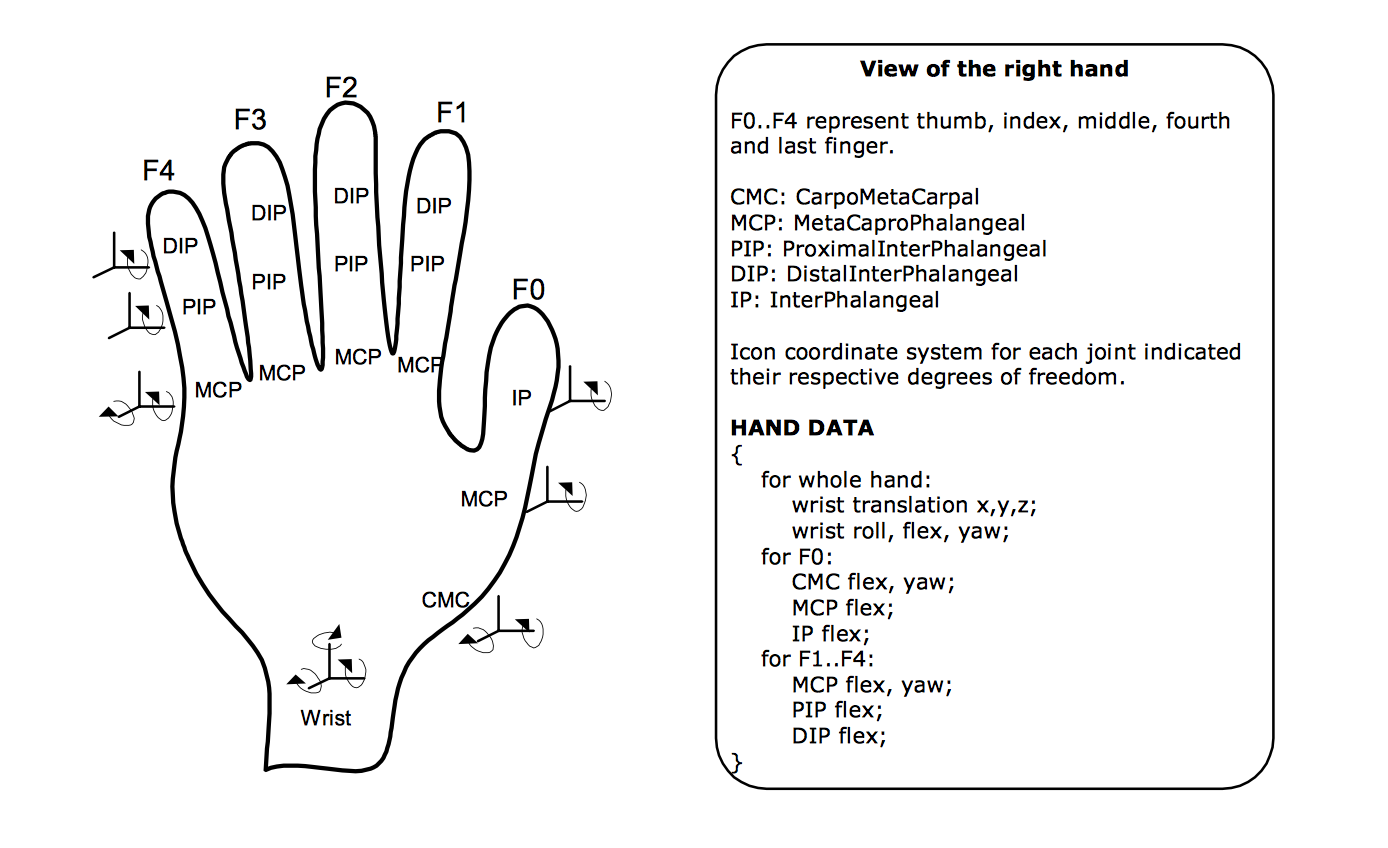
\includegraphics[scale=0.47]{hand-dof.png}
  \caption{General model of the hand}
  \end{figure}
  
  Next step is to locate so-called "palm point", the center point of the palm, which will help us to identify the palm, segment it and determine orientation of the hand. To do that, we can use a distance tranform algorithm, where the matrix of the same size is filled with distances to the closest pixel boundary. The point with $max(d)$ is defined to be a palm point.\\
  \\
  Now, let's draw a circle around this point, increasing radius every time until non-skin values appear. Such a circle with a maximal radius will encompass the entire palm and is called inner circle. Once we've determined that, we draw another circle, with the radius of 1.2 times the inner circle's one \cite{ZH01}. To eliminate the non-skin regions and trace the hand more carefully, points are sampled across the circle and lined up with their closest boundary neighbors. This larger circle will function as a palm mask, allowing us to easily separate the image into palm and fingers. Everything below the wrist line (parts of the arm) will be removed to minimize interference and the produced hand image will be rotated to the point where wrist line is parallel to $x$ axis.\\
  \\
  The result of this step is illustrated at the image below (taken from \cite{ZH01}):\\
  
   \begin{figure}[H]
  \centering
  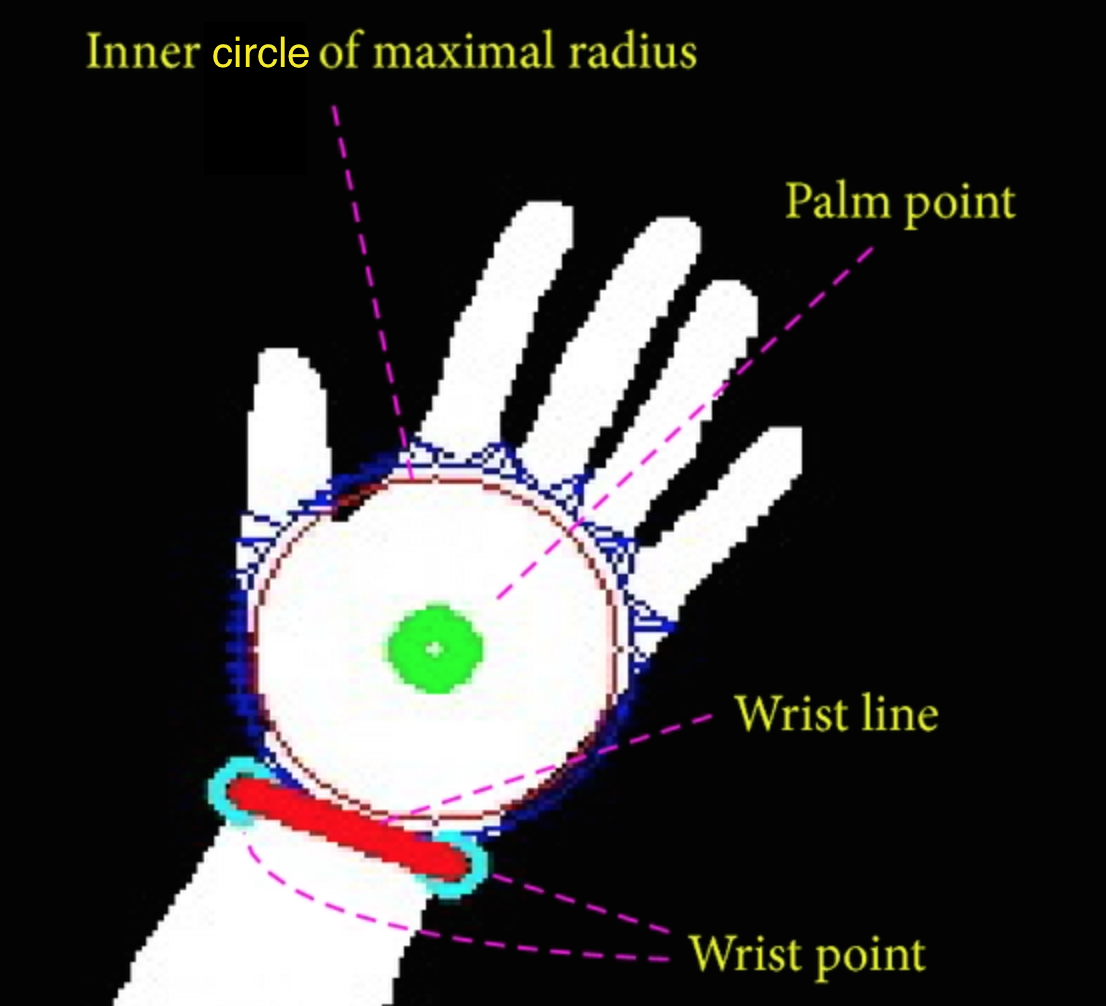
\includegraphics[scale=0.35]{hand-segmentation.png}
  \caption{Post-processing results}
  \end{figure}
  
  \subsection{Finger recognition}
  
	After segmenting the palm from the image, we will be left with separately recognized fingers, that are visible to the sensor. Each finger then is bounded by a rectangle, a center of which we will call a center point of a finger. We connect each one of those points to the palm point and calculate the degree between the formed lines and a wrist line. If we find a line with $\alpha < 50\degree$, we can say that it's a thumb and mark it a such (with index $i=0$). If there is no line with $\alpha > 50\degree$, we can judge that a thumb is not visible on an image. To recognize the other fingers, we can draw a line above palm point, which is parallel to the wrist line (let's call it palm line). Then, using center points of the fingers, we can classify which finger is which, based on horizontal coordinate with respect to plam line, separated in 4 segments of roughly the same size. In some cases, however, due to poor resolution, two or more fingers may be mixed together in a single blob. In that case, we can use the width of the bounding rectangle as an indicator whether multiple fingers have been merged. After processing, roughly the following image will be formed (taken from \cite{ZH01}):
    
  \begin{figure}[H]
  \centering
  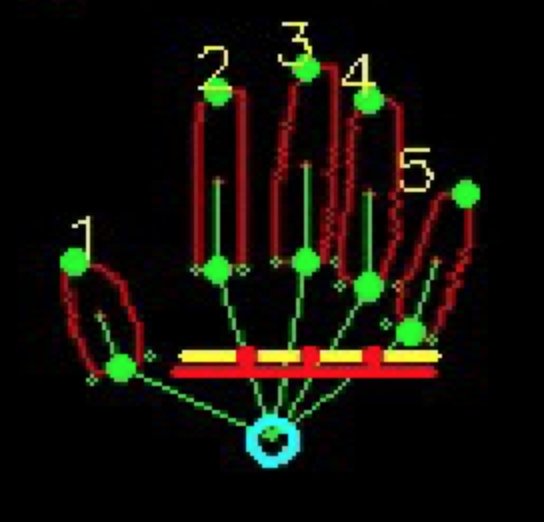
\includegraphics[scale=0.7]{hand-recognized.png}
  \caption{Model after finger recognition}
  \end{figure}
 
  \subsection{Gesture set}
	
    The following basic gesture set has been selected for the purposes of this project. Default semantics of those gestures are described, and the basic actions are assigned to them, based on some of the suggestions presented in CADDIAN language draft \cite{AB01}. Let's separate all the gestures into two kinds: \textbf{static}, corresponding to a single hand expression and \textbf{dynamic},  building upon the static ones, but also tracking hand animation (such as movement or a sequence of changing states). This list is meant only as the initial draft and should be easily extensible, once more features are needed.
    
    \subsubsection{Static gestures}
    
  \begin{figure}[H]
  \centering
  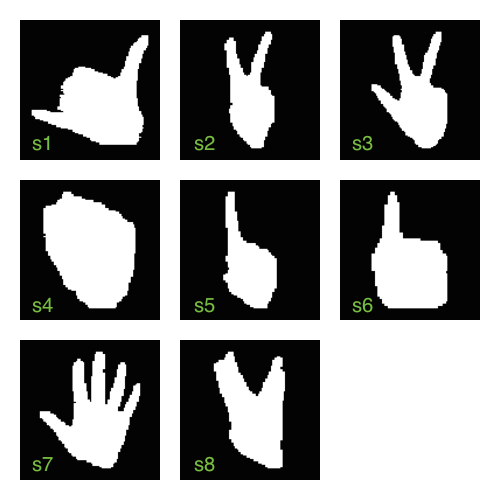
\includegraphics[scale=0.4]{static-gestureset.png}
  \caption{Static gesture set}
  \end{figure}
    
    \begin{itemize}
    \item \textbf{s1.} Ascend. The longer user keeps the gesture, bigger the priority.
    \item \textbf{s2.} Descend. The longer user keeps the gesture, bigger the priority.
    \item \textbf{s3.} Turn $90\degree$ to the right.
    \item \textbf{s4.} Turn $90\degree$ to the left.
    \item \textbf{s5.} Confirm action / Accellerate.
    \item \textbf{s6.} Cancel action / Decellerate.
    \item \textbf{s7.} Switch between piloting and task management (for gestures s6 and s7).
    \item \textbf{s8.} Predator (for example, shark) has been spotted, use caution.
    \item \textbf{s9.} Abort the current operation.
    \item \textbf{s10.} Contact the crew with operation logs and message from the diver.
    \item \textbf{s11.} Take a picture.
    \item \textbf{s12.} Take a picture and a 3D scan of surrounding area.
    \end{itemize}
    
    \subsubsection{Dynamic gestures}
    
  \begin{figure}[H]
  \centering
  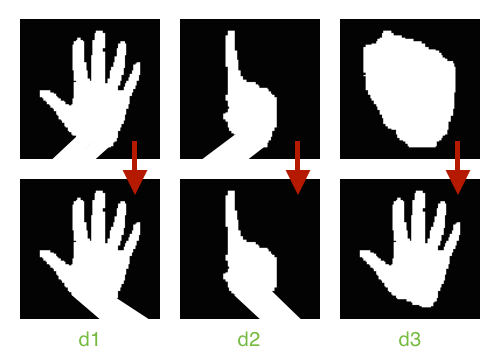
\includegraphics[scale=0.5]{dynamic-gestureset.png}
  \caption{Dynamic gesture set}
  \end{figure}
  
  \begin{itemize}
    \item \textbf{d1.} Emergency. Immediate abort of operations and ascend are requested. Faster the movement, bigger the priority.
    \item \textbf{d2.} Warning. Pause the operation and analyze the surroundings, contact the crew. Faster the movement, bigger the priority.
    \item \textbf{d3.} Closing and opening fist rapidly. Indicates that the oxygen is running out.
    \end{itemize}

  \subsection{Recognizing static gestures}
  
 Now that we can detect and identify individual fingers, static gestures can be recognized with a simple rule classifier. In this case, the hand gesture can be predicted, based on the number and indexes of the visible fingers. For example, if two fingers, index and middle one, are visible, gesture \textbf{s8} will be recognized.\\
 \\
 In some of the cases (like \textbf{s1/s2} and \textbf{s5/s6}), the direction vector will be determined with regards to the wrist line, to determine which action needs to be performed. Additionally, since both hands are being tracked at the same time, more complex gestures can be defined using the combination of two hands (here, \textbf{s9}).
  
  \subsection{Recognizing dynamic gestures}
  
  Dynamic gestures are built upon the methods used to recognize static gestures, however it is not enough to describe the motion. Therefore, each particular dynamic gesture will have its own detection function, based on the number of applicable parameters.\\
  \\
  We start by recognizing a hand expression and checking whether it corresponds to the initial (staring) state of any of the dynamic gestures. If it does, the function is executed, which checks in the consecutive following frames, whether the conditions for the gesture have been met. For the gestures \textbf{d1} and \textbf{d2}, for example, the global $x$-position of the hand will be monitored. If no movement of a sufficient offset was detected before timeout $t$, the corresponding static gesture (if any) will be executed. However, if hand movement is detected, a timer for the minimum duration of the gesture is setup and hand position is continued to be analyzed. If back-and-forth movement continues with defined offsets, a dynamic gesture is recognized. Based on the intensity of the movement (which can be calculated using hand offset and timestamps of the frames), priority is being assigned to the task.\\
  \\
  Some of the dynamic gestures, however, don't require moving hands. In our gesture set, \textbf{d3} will consist of no movement, but rapid changing of hand expressions. In this case, similarly, after recognizing the initial hand expression, the function will check whether the state altered within some timeout $t$. Choosing sufficiently small timeout value will allow our robot to detect gestures in general without critical pauses in between, but watch out for the dynamics of the gesture as well.
  
  \subsection{Code License}
  
  All the code, written as the part of this research project will be available under \textbf{GPL v2} license. Code will be available freely as an open-source repository hosted on Github. Anyone is free to use, modify or distribute this software and its parts, as long as they provide an attribution back and license it under the same terms.
  
  \subsection{Testing}
  
  Test suite will be created for every component of the application. Complexity of the tests will vary from the simple ones (to check if Kinect is properly recognized or to be sure than hand segmentation actually works) to more complex ones (feeding a set of images with gestures to see if the correct one is identified). More than that, over the course of development I will adhere to \textbf{test-driven development} to minimize the time spent on fixing bugs and narrowing the source of potential problems.

  \section{Timeline}

  \begin{tabular}{|c|c|}
  \hline
  \textbf{Time Span} & \textbf{Activity} \\ \hline
  01/09/2014 - 01/10/2014 & Defining a research topic \\ \hline
  01/10/2014 - 01/11/2014 & Searching for related literature \\ \hline
  01/11/2014 - 05/12/2014 & Preparing a research proposal \\ \hline
  05/12/2014 - 23/12/2014 & Implementing hand segmentation and finger recognition \\ \hline
  23/12/2014 - 11/01/2015 & Holiday \\ \hline
  12/01/2015 - 18/02/2015 & Implementing gesture recognizer based on the defined gesture set \\ \hline
  19/02/2015 - 03/03/2015 & Writing tests and fixing bugs \\ \hline
  04/03/2015 - 10/03/2015 & Final corrections \\ \hline
  10/03/2015 - 10/03/2015 & BSc Thesis presentation \\ \hline
  \end{tabular}

  \section{Deliverable}
  
  The final deliverable of this project will be an application, that displays video stream from Kinect sensor and highlights recognized gestures. Overall, code should be modular, easily adaptable and ready to include in the side projects or deploy in the real world.
  
  \section{Conclusion}

  Summarizing all the information presented above, we can see that gesture recognition, despite being a pretty novel technology, has a lot of useful applications. In our case, communicating with robot underwater can be complicated due to a number of natural events. Gesture recognition system allows to control the robot from the safe distance and keep track of health conditions of the diver. Step-by-step approach to gesture recognition was presented, starting from hand segmentation and ending with identifying different kinds of gestures. Finally, organizational matters like code license, project timeline and final deliverables were discussed.
  
  \section{Evaluation Criteria}
  
  Evaluation criteria for this research project are strongly coupled with the project requirements and implementation quality. The following criteria can be distinguished and used to evaluate the results of this thesis:
  
  \begin{itemize}
  \item \textbf{Functionality.} Application is able to recognize and process the gestures from a pre-defined set. 
  \item \textbf{Correctness.} Application doesn't trigger on undefined gestures and doesn't mix gestures up.
   \item \textbf{Modularity.} Application is easily extensible to add more gestures or change the trigger functions. 
  \item \textbf{Code Quality.} Consistent style of coding is maintained. Source code is factored and organized well.
  \item \textbf{Documentation.} Source code and underlying mathematical principles are documented well.
  \item \textbf{Testing.} Every logical part of the application is tested separately on a number of test cases. 
  \end{itemize}
  
  \section{Acknowledgements}
  I would like to thank Prof. Andreas Birk for the advice and assistance in the course of working on this thesis and Prof. Horst Hahn for his excellent course in image processing. I would also like to thank Microsoft for providing me with Kinect sensor over the course of my internship. Finally, there is no way I would reach where I am now without my family and friends - I thank them for their support and for making me the person, that I am today.

  \newpage
  \renewcommand{\refname}{\section{References}}
  
  \bibliographystyle{unsrt}
  \bibliography{thesis}

\end{document}